\documentclass[12pt,a4paper,oneside]{book}

% ---------- Geometry & core packages ----------
\usepackage[a4paper,top=2.7cm,bottom=2.7cm,left=3.0cm,right=2.5cm,bindingoffset=0.4cm]{geometry}
\usepackage[utf8]{inputenc}
\usepackage[T1]{fontenc}
\usepackage{amsmath}
\usepackage{amssymb}
\usepackage[table]{xcolor}
\usepackage{booktabs}
\usepackage{array}
\usepackage{tabularx}
\usepackage{enumitem}
\usepackage{titlesec}
\usepackage{fancyhdr}
\usepackage{setspace}
\usepackage{caption}
\usepackage{tikz}
\usetikzlibrary{positioning,calc,shapes.geometric,decorations.pathmorphing,backgrounds,patterns}
\usepackage[skins,breakable]{tcolorbox}
\usepackage{fontawesome5}
\usepackage{hyperref}

% ---------- Palette ----------
\definecolor{monashblue}{RGB}{0,56,101}
\definecolor{monashteal}{RGB}{0,131,138}
\definecolor{sandgold}{RGB}{188,143,58}
\definecolor{papergray}{RGB}{246,247,248}

\hypersetup{
  colorlinks=true,
  linkcolor=monashblue,
  citecolor=monashteal,
  urlcolor=monashteal,
  pdftitle={Adaptive Model Predictive Control for Resilient Operation of Distributed Renewable Microgrids},
  pdfauthor={Aisha Rahman}
}

% ---------- Heading styles ----------
\titleformat{\chapter}[display]
  {\normalfont\huge\bfseries\color{monashblue}}
  {\filright\Large\color{monashteal}\chaptertitlename\ \thechapter}
  {8pt}{\Huge\raggedright}
\titlespacing*{\chapter}{0pt}{10pt}{30pt}

\titleformat{\section}
  {\normalfont\Large\bfseries\color{monashblue}}{\thesection}{0.8em}{}
\titleformat{\subsection}
  {\normalfont\large\bfseries\color{monashteal}}{\thesubsection}{0.8em}{}

% ---------- Headers & footers ----------
\setlength{\headheight}{24.1pt}
\pagestyle{fancy}
\fancyhf{}
\fancyhead[L]{\small\itshape\nouppercase{\leftmark}}
\fancyhead[R]{\small\itshape\nouppercase{\rightmark}}
\fancyfoot[C]{\small\thepage}
\renewcommand{\headrulewidth}{0.4pt}
\renewcommand{\headrule}{\hbox to\headwidth{\color{monashteal}\leaders\hrule height \headrulewidth\hfill}}
\renewcommand{\chaptermark}[1]{\markboth{\thechapter.\ #1}{}}
\renewcommand{\sectionmark}[1]{\markright{\thesection.\ #1}}

\fancypagestyle{plain}{%
  \fancyhf{}
  \fancyfoot[C]{\small\thepage}
  \renewcommand{\headrulewidth}{0pt}
}

\onehalfspacing
\setlength{\parskip}{4pt}

% ---------- tcolorbox styles ----------
\tcbset{
  infobox/.style={
    colback=monashblue!4, colframe=monashblue, boxrule=0.6pt,
    left=8pt, right=8pt, top=6pt, bottom=6pt,
    fonttitle=\bfseries\color{white}, coltitle=white,
    colbacktitle=monashblue, title={#1}
  }
}

\begin{document}

% ============================================================
% TITLE PAGE
% ============================================================
\begin{titlepage}
\thispagestyle{empty}
\begin{tikzpicture}[remember picture, overlay]
  \fill[monashblue] (current page.north west) rectangle ([xshift=0.9cm]current page.south west);
  \begin{scope}[on background layer]
    \fill[pattern=dots, pattern color=monashblue!15]
      ([xshift=-6cm,yshift=-6cm]current page.north east) rectangle (current page.north east);
  \end{scope}
\end{tikzpicture}

\vspace*{0.3cm}
\hspace*{0.6cm}
\begin{minipage}{0.86\textwidth}
{\small\bfseries\color{monashteal} FACULTY OF ENGINEERING}\\[2pt]
{\small\color{monashblue} Department of Electrical and Computer Systems Engineering}
\end{minipage}
\par

\vspace{0.8cm}
\hspace*{0.6cm}
\begin{minipage}{0.86\textwidth}
\centering

\begin{tikzpicture}
  \begin{scope}[on background layer]
    \fill[monashblue!6] (-1.1,-0.9) rectangle (1.6,0.9);
  \end{scope}
  \node[regular polygon, regular polygon sides=6, draw=monashblue, thick,
        minimum size=1.5cm, fill=monashblue!12] (hex) at (0,0) {};
  \node[circle, draw=sandgold, thick, fill=sandgold!20, minimum size=1.0cm] (circ) at (0.45,0.3) {};
\end{tikzpicture}
\end{minipage}
\par

\vspace{0.5cm}
\hspace*{0.6cm}
\begin{minipage}{0.86\textwidth}
\centering
\begin{tikzpicture}
  \draw[monashteal, thick, decorate, decoration={snake, amplitude=0.5mm, segment length=4mm}]
    (0,0) -- (9.5,0);
\end{tikzpicture}

\vspace{0.3cm}
{\huge\bfseries\color{monashblue} Adaptive Model Predictive Control for Resilient Operation of Distributed Renewable Microgrids}

\vspace{0.6cm}
{\large\itshape\color{monashteal} A data-driven framework for uncertainty-aware\\ energy management in low-inertia power networks}
\end{minipage}
\par

\vspace{0.8cm}
\hspace*{0.6cm}
\begin{minipage}{0.86\textwidth}
\centering
{\Large Aisha Rahman}\\[4pt]
{\small\itshape Bachelor of Engineering (Hons.), Master of Engineering Science}
\end{minipage}
\par

\vspace{0.7cm}
\hspace*{0.6cm}
\begin{minipage}{0.86\textwidth}
\centering
\begin{tcolorbox}[width=0.92\linewidth, colback=papergray, colframe=monashblue!40,
  boxrule=0.5pt, arc=2pt, left=10pt, right=10pt, top=8pt, bottom=8pt]
\small
\begin{tabular}{@{}ll@{}}
\faFile\ \textbf{Degree:} & Doctor of Philosophy \\
\faCalendar\ \textbf{Submitted:} & February 2026 \\
\end{tabular}
\end{tcolorbox}
\end{minipage}
\par

\vspace{0.6cm}
\hspace*{0.6cm}
\begin{minipage}{0.86\textwidth}
\centering
\small
A thesis submitted for the degree of Doctor of Philosophy at\\
\textbf{Monash University} in 2026\\
Department of Electrical and Computer Systems Engineering
\end{minipage}
\par

\vfill
\hspace*{0.6cm}
\begin{minipage}{0.86\textwidth}
\centering
{\footnotesize\itshape\color{monashblue!70} Unofficial template --- not affiliated with or endorsed by the university. Sample content only.}
\end{minipage}
\vspace{0.4cm}

\end{titlepage}

\frontmatter

% ============================================================
% COPYRIGHT NOTICE
% ============================================================
\chapter*{Copyright Notice}
\addcontentsline{toc}{chapter}{Copyright Notice}
\markboth{Copyright Notice}{Copyright Notice}

\noindent \copyright\ Aisha Rahman, 2026.

\vspace{0.4cm}
\noindent I certify that I have made all reasonable efforts to secure copyright permissions for third-party content included in this thesis and have not knowingly added copyright content to my work without the owner's permission.

\vspace{0.4cm}
\noindent Except as provided in the \emph{Copyright Act 1968}, this thesis may not be reproduced in any form without the written permission of the author.

\vspace{0.4cm}
\noindent I retain all proprietary rights, such as patent rights. I also retain the right to use in future works (such as articles or books) all or part of this thesis.

% ============================================================
% ABSTRACT
% ============================================================
\chapter*{Abstract}
\addcontentsline{toc}{chapter}{Abstract}
\markboth{Abstract}{Abstract}

The accelerating integration of photovoltaic (PV) generation and battery energy storage systems (BESS) into distribution networks is displacing conventional synchronous generation, reducing system inertia and exposing microgrids to increased operational volatility. Existing rule-based and single-horizon optimisation controllers struggle to reconcile short-term forecast uncertainty with long-term degradation and reliability objectives, particularly during islanded operation following upstream network disturbances.

This thesis develops and validates an adaptive model predictive control (MPC) framework for resilient microgrid energy management under deep renewable penetration. The framework couples a rolling-horizon optimisation core with an online forecast-error correction layer, allowing the controller to reweight state-of-charge (SOC) reserve margins in response to observed prediction drift rather than relying on static safety factors. A reduced-order thermal-electrochemical battery model is embedded within the optimisation to jointly minimise operating cost and cumulative degradation.

The proposed controller is evaluated against baseline rule-based and static-horizon MPC strategies using twelve months of half-hourly irradiance, load, and tariff data drawn from a synthetic feeder representative of regional Australian conditions. Across all evaluated scenarios, the adaptive controller reduces expected daily operating cost by 14.2\% relative to the rule-based baseline and by 6.8\% relative to static-horizon MPC, while reducing SOC constraint violations during islanding events by more than half. Computation time remains within the bounds required for five-minute dispatch cycles on embedded controller hardware.

These results indicate that explicitly modelling and correcting for forecast uncertainty within the control loop -- rather than treating it as an external disturbance -- yields measurable gains in both economic performance and operational resilience. The thesis contributes a generalisable adaptive-horizon formulation, an open evaluation methodology for islanding resilience, and a set of design guidelines for practitioners deploying MPC-based controllers on resource-constrained microgrid hardware.

% ============================================================
% DECLARATION
% ============================================================
\chapter*{Declaration}
\addcontentsline{toc}{chapter}{Declaration}
\markboth{Declaration}{Declaration}

This thesis is an original work of my research and contains no material which has been accepted for the award of any other degree or diploma at any university or equivalent institution. To the best of my knowledge, this thesis contains no material previously published or written by another person, except where due reference is made in the text.

\vspace{1.2cm}
\noindent
\begin{tabular}{@{}ll@{}}
Print Name: & Aisha Rahman \\[6pt]
Date: & 12 February 2026 \\
\end{tabular}

% ============================================================
% ACKNOWLEDGEMENTS
% ============================================================
\chapter*{Acknowledgements}
\addcontentsline{toc}{chapter}{Acknowledgements}
\markboth{Acknowledgements}{Acknowledgements}

I am deeply grateful to my principal supervisor, Professor Daniel Whitfield, for his rigorous feedback, patience, and consistent encouragement throughout the candidature, and to my associate supervisor, Dr Priya Nandakumar, whose expertise in power system dynamics shaped the direction of the control formulation in Chapter~3.

I thank the members of the Distributed Energy Systems research group for numerous discussions that improved the clarity of this work, and the technical staff who supported the feeder emulation testbed used to validate the controller. Financial support from the Nimbus Foundation Scholarship is gratefully acknowledged.

Finally, I thank my family, and in particular my partner Tom, for their patience and support over the course of this candidature.

% ============================================================
% TOC / LOF / LOT / ABBREVIATIONS
% ============================================================
\tableofcontents
\listoffigures
\listoftables

\chapter*{List of Abbreviations}
\addcontentsline{toc}{chapter}{List of Abbreviations}
\markboth{List of Abbreviations}{List of Abbreviations}

\begin{center}
\renewcommand{\arraystretch}{1.25}
\begin{tabularx}{0.85\textwidth}{@{}l X@{}}
\toprule
\rowcolor{monashblue!10}
\textbf{Abbreviation} & \textbf{Meaning} \\
\midrule
BESS & Battery Energy Storage System \\
DER  & Distributed Energy Resource \\
MPC  & Model Predictive Control \\
PV   & Photovoltaic \\
RES  & Renewable Energy Source \\
SOC  & State of Charge \\
THD  & Total Harmonic Distortion \\
RMSE & Root Mean Square Error \\
\bottomrule
\end{tabularx}
\end{center}

\mainmatter

% ============================================================
% CHAPTER 1 -- INTRODUCTION
% ============================================================
\chapter{Introduction}
\label{ch:introduction}

\section{Background}

Distribution networks worldwide are undergoing a rapid shift from centralised, synchronous generation towards distributed, inverter-interfaced renewable resources. Rooftop and community-scale PV, paired increasingly with BESS, now supply a substantial share of local demand in many regional feeders. While this transition delivers clear decarbonisation benefits, it also reduces the physical inertia and short-circuit strength that conventional generators historically provided, leaving feeders more sensitive to fast disturbances and forecast error.

Microgrids -- localised clusters of generation, storage, and load capable of operating connected to, or islanded from, the upstream grid -- are widely viewed as a practical response to this challenge. Their value proposition rests on the quality of the underlying energy management system: a controller that dispatches generation and storage to minimise cost while preserving enough operational headroom to withstand disturbances, including unplanned islanding.

\section{Problem Statement}

Two dominant control paradigms are used in practice. Rule-based controllers are robust and computationally trivial but leave significant economic value unrealised, since fixed thresholds cannot adapt to time-varying conditions. Model predictive control improves on this by solving a rolling-horizon optimisation against a forecast, but conventional formulations treat the forecast as exact within the horizon and rely on static reserve margins to absorb error. When forecast error is systematically underestimated -- for example during rapidly changing cloud cover -- static margins are either too conservative, eroding economic performance, or too thin, exposing the system to SOC violations precisely when resilience matters most.

\begin{tcolorbox}[infobox={Research Objectives}]
\begin{enumerate}[label=\textbf{O\arabic*.}, leftmargin=2.2em]
  \item Develop a rolling-horizon MPC formulation that adapts SOC reserve margins online, using observed forecast-error statistics rather than fixed safety factors.
  \item Embed a computationally tractable battery degradation model within the optimisation to jointly manage cost and long-run asset health.
  \item Evaluate the resulting controller's economic performance and islanding resilience against established baselines using a full-year, half-hourly case study.
\end{enumerate}
\end{tcolorbox}

\section{Research Questions}

This thesis addresses three research questions:

\begin{itemize}[leftmargin=2.2em]
  \item[\textbf{RQ1.}] How should forecast-error statistics be incorporated into the MPC reserve-margin calculation without materially increasing solve time?
  \item[\textbf{RQ2.}] What is the trade-off between economic performance and islanding resilience as reserve-margin adaptivity increases?
  \item[\textbf{RQ3.}] Does the resulting controller remain deployable on embedded hardware operating at typical five-minute dispatch cycles?
\end{itemize}

\section{Conceptual Framework}

Figure~\ref{fig:framework} summarises the conceptual framework developed in this thesis, linking a data layer (sensing and forecasting), a control layer (the adaptive MPC core), and a physical layer (DERs and loads), with feedback from observed physical outcomes correcting the data layer's error model.

\begin{figure}[htbp]
\centering
\begin{tikzpicture}[
  box/.style={rectangle, rounded corners, draw=monashblue, thick, fill=monashblue!8,
              minimum width=3.1cm, minimum height=1.5cm, align=center, font=\small},
]
\node[box] (data) {Data Layer\\{\footnotesize Sensing \& Forecasting}};
\node[box, right=1.7cm of data] (ctrl) {Control Layer\\{\footnotesize Adaptive MPC}};
\node[box, right=1.7cm of ctrl] (phys) {Physical Layer\\{\footnotesize DERs \& Loads}};
\draw[->, thick, monashteal] (data) -- (ctrl);
\draw[->, thick, monashteal] (ctrl) -- (phys);
\draw[->, thick, monashteal, dashed] (phys.south) .. controls +(0,-1.1) and +(0,-1.1) .. (data.south);
\node[font=\footnotesize, below=0.05cm of data, xshift=1.9cm, yshift=-0.85cm, monashteal] {error feedback};
\end{tikzpicture}
\caption{Conceptual framework linking data, control, and physical layers.}
\label{fig:framework}
\end{figure}

\section{Thesis Outline}

Table~\ref{tab:outline} maps the remaining chapters of this thesis to their primary focus.

\begin{table}[htbp]
\centering
\caption{Thesis structure overview.}
\label{tab:outline}
\renewcommand{\arraystretch}{1.3}
\begin{tabularx}{\textwidth}{@{}l X@{}}
\toprule
\rowcolor{monashblue!10}
\textbf{Chapter} & \textbf{Focus} \\
\midrule
2. Literature Review & Positions this work relative to microgrid control architectures and forecast-aware MPC. \\
3. Methodology & Presents the system model, adaptive MPC formulation, and evaluation design. \\
4. Results and Discussion & Reports comparative performance across baseline, static-horizon, and adaptive controllers. \\
5. Conclusion & Summarises contributions, limitations, and directions for future work. \\
\bottomrule
\end{tabularx}
\end{table}

% ============================================================
% CHAPTER 2 -- LITERATURE REVIEW
% ============================================================
\chapter{Literature Review}
\label{ch:literature}

\section{Microgrid Control Architectures}

Microgrid control is conventionally organised in a hierarchical structure spanning primary droop control, secondary restoration, and tertiary economic dispatch. This thesis is concerned with the tertiary layer, where the controller determines setpoints for BESS charge/discharge and curtailable load over a rolling horizon of minutes to hours.

\section{Model Predictive Control in Power Systems}

MPC has been applied extensively to microgrid dispatch because it naturally accommodates constraints on SOC, ramp rates, and grid import limits while optimising an explicit cost function. Early formulations solved a deterministic optimisation against a single point forecast, a design choice inherited from industrial process control settings where forecast uncertainty is comparatively small. Subsequent work introduced scenario-based and chance-constrained variants to hedge against forecast error, generally at substantial computational cost.

\section{Uncertainty and Forecasting}

A parallel body of work focuses on improving the point forecasts feeding into the controller, using statistical and learning-based methods, rather than modifying how the controller consumes forecast uncertainty once available. Comparatively little work has examined online adaptation of the controller's own reserve margins as a function of realised forecast error, which is the gap this thesis addresses.

\section{Research Gap}

Table~\ref{tab:litreview} summarises representative studies and their treatment of forecast uncertainty.

\begin{table}[htbp]
\centering
\caption{Representative prior approaches to microgrid MPC.}
\label{tab:litreview}
\renewcommand{\arraystretch}{1.3}
\begin{tabularx}{\textwidth}{@{}l l X X@{}}
\toprule
\rowcolor{monashblue!10}
\textbf{Study} & \textbf{Year} & \textbf{Control Approach} & \textbf{Key Limitation} \\
\midrule
Okafor \& Lindqvist & 2021 & Deterministic single-horizon MPC & Static reserve margins; no error feedback \\
Zhao et al.         & 2022 & Scenario-based stochastic MPC & High solve time; unsuitable for embedded dispatch \\
Herrera \& Novak     & 2023 & Chance-constrained MPC & Fixed confidence level; ignores forecast drift \\
Petrov et al.        & 2024 & Learning-augmented forecasting & Improves forecasts only; controller unchanged \\
\bottomrule
\end{tabularx}
\end{table}

The reviewed literature either improves forecast accuracy or hedges against uncertainty with static margins, but none adapts reserve margins online using realised forecast-error statistics -- the contribution developed in Chapter~3.

% ============================================================
% CHAPTER 3 -- METHODOLOGY
% ============================================================
\chapter{Methodology}
\label{ch:methodology}

\section{System Architecture}

The candidate microgrid comprises a PV array, a lithium-ion BESS, an aggregated local load, and a point of common coupling with the utility grid, coordinated by the proposed adaptive MPC controller. Figure~\ref{fig:architecture} illustrates the information flow between components.

\begin{figure}[htbp]
\centering
\begin{tikzpicture}[
  comp/.style={rectangle, rounded corners, draw=monashblue, thick, fill=white,
               minimum width=2.7cm, minimum height=1.1cm, align=center, font=\small},
  ctrl/.style={rectangle, rounded corners, draw=sandgold, thick, fill=sandgold!12,
               minimum width=3.4cm, minimum height=1.3cm, align=center, font=\small\bfseries}
]
\node[comp] (pv) {PV Array};
\node[comp, below=0.9cm of pv] (bess) {Battery Storage};
\node[comp, below=0.9cm of bess] (load) {Local Load};
\node[ctrl, right=2.8cm of bess] (mpc) {Adaptive MPC\\ Controller};
\node[comp, right=2.8cm of mpc] (grid) {Utility Grid};
\draw[->, thick] (pv) -- (mpc);
\draw[->, thick] (bess) -- (mpc);
\draw[->, thick] (load) -- (mpc);
\draw[->, thick] (mpc) -- (grid);
\draw[->, thick, monashteal, dashed] (mpc.north) to[bend left=30] (bess.east);
\end{tikzpicture}
\caption{System architecture: information and setpoint flow between components.}
\label{fig:architecture}
\end{figure}

\section{Adaptive MPC Formulation}

At each dispatch step $k$, the controller solves a finite-horizon optimisation over horizon length $N$, minimising expected operating cost subject to power balance, SOC, and ramp constraints:

\begin{equation}
\min_{\{p_t\}} \; \sum_{t=k}^{k+N-1} \Big( c_t\, p^{\text{grid}}_t + \lambda\, d_t \Big)
\label{eq:objective}
\end{equation}

\begin{equation}
\text{s.t.} \quad \mathrm{SOC}_{t+1} = \mathrm{SOC}_t + \eta\, p^{\text{batt}}_t \,\Delta t, \qquad
\mathrm{SOC}^{\min}_t \le \mathrm{SOC}_t \le \mathrm{SOC}^{\max}_t
\label{eq:soc}
\end{equation}

where $c_t$ is the time-varying import tariff, $d_t$ the incremental battery degradation cost, $\lambda$ a weighting parameter, and $\mathrm{SOC}^{\min}_t$, $\mathrm{SOC}^{\max}_t$ the reserve-adjusted state-of-charge bounds. The key contribution of this thesis is that $\mathrm{SOC}^{\min}_t$ is not fixed but is recomputed at every step as a function of the exponentially weighted forecast-error variance observed over the preceding $W$ steps, tightening the margin only when recent forecasts have proven unreliable.

\section{Case Study and Data}

The controller is evaluated using twelve months of synthetic half-hourly irradiance, load, and tariff data constructed to be representative of a regional Australian feeder. Table~\ref{tab:dataset} summarises the key case-study parameters.

\begin{table}[htbp]
\centering
\caption{Case study parameters.}
\label{tab:dataset}
\renewcommand{\arraystretch}{1.3}
\begin{tabularx}{\textwidth}{@{}l X@{}}
\toprule
\rowcolor{monashblue!10}
\textbf{Parameter} & \textbf{Value} \\
\midrule
Simulation horizon & 12 months, 30-minute resolution \\
PV capacity & 250 kWp \\
BESS capacity & 400 kWh, 200 kW \\
Peak local load & 310 kW \\
Grid import limit & 350 kW \\
Optimisation horizon $N$ & 48 steps (24 hours) \\
Dispatch interval & 5 minutes (re-solved each step) \\
\bottomrule
\end{tabularx}
\end{table}

\section{Evaluation Metrics}

Controllers are compared on four metrics: expected daily operating cost, frequency of SOC constraint violations during simulated islanding events, cumulative battery degradation cost, and mean per-step solve time. All scenarios are repeated across three seasonal profiles (summer, winter, shoulder) to assess sensitivity to irradiance variability.

% ============================================================
% CHAPTER 4 -- RESULTS AND DISCUSSION
% ============================================================
\chapter{Results and Discussion}
\label{ch:results}

\section{Comparative Performance}

Table~\ref{tab:results} reports aggregate performance across the three seasonal profiles for the rule-based baseline, static-horizon MPC, and the proposed adaptive MPC controller.

\begin{table}[htbp]
\centering
\caption{Comparative performance across controllers (annual average).}
\label{tab:results}
\renewcommand{\arraystretch}{1.3}
\begin{tabularx}{\textwidth}{@{}l X X X@{}}
\toprule
\rowcolor{monashblue!10}
\textbf{Metric} & \textbf{Rule-Based} & \textbf{Static MPC} & \textbf{Adaptive MPC} \\
\midrule
Daily operating cost (relative) & 100.0\% & 92.3\% & 85.8\% \\
SOC violations per islanding event & 3.4 & 1.9 & 0.8 \\
Degradation cost (relative) & 100.0\% & 97.1\% & 91.4\% \\
Mean solve time (ms) & --- & 41 & 58 \\
\bottomrule
\end{tabularx}
\end{table}

\section{Discussion}

The adaptive controller reduces expected daily operating cost by 14.2\% relative to the rule-based baseline and by 6.8\% relative to static-horizon MPC, driven primarily by tighter SOC margins during periods of high forecast confidence. SOC violations during islanding events fall by more than half relative to static-horizon MPC, indicating that the adaptive margin correctly widens ahead of periods of elevated forecast error, such as the onset of rapidly moving cloud cover.

The 17-millisecond increase in mean solve time relative to static-horizon MPC remains well within the budget available for five-minute dispatch cycles on the embedded controller hardware used in this study, addressing RQ3. The residual gap between adaptive and theoretical perfect-foresight performance -- not shown in Table~\ref{tab:results} -- suggests that further gains are available from improving the underlying forecast model itself, a direction discussed in Chapter~5.

% ============================================================
% CHAPTER 5 -- CONCLUSION
% ============================================================
\chapter{Conclusion and Future Work}
\label{ch:conclusion}

\section{Summary of Contributions}

This thesis developed an adaptive model predictive control framework that incorporates online forecast-error correction into microgrid energy management, addressing a gap in existing MPC formulations that rely on static reserve margins. The framework was validated using a full-year case study representative of a regional Australian feeder, demonstrating simultaneous improvements in economic performance and islanding resilience relative to established baselines.

\begin{tcolorbox}[infobox={Key Contributions}]
\begin{itemize}[leftmargin=1.6em]
  \item An adaptive reserve-margin formulation driven by exponentially weighted forecast-error variance.
  \item A tractable embedded battery degradation model suitable for rolling-horizon optimisation.
  \item An evaluation methodology for islanding resilience applicable beyond the specific case study presented.
\end{itemize}
\end{tcolorbox}

\section{Limitations}

The evaluation relies on synthetic rather than field-measured feeder data, and the degradation model, while computationally tractable, is a reduced-order approximation of full electrochemical behaviour. Results should therefore be interpreted as indicative of relative controller performance rather than absolute field-deployable figures.

\section{Future Work}

Future work should validate the controller against field data from an instrumented feeder, extend the formulation to coordinate multiple interconnected microgrids, and investigate learning-based forecast models that could be jointly trained with the reserve-margin adaptation rule described in Chapter~3.

\backmatter

% ============================================================
% APPENDIX
% ============================================================
\appendix
\chapter{Supplementary Controller Parameters}
\label{app:parameters}

Table~\ref{tab:appendix} lists the controller tuning parameters used across all reported experiments.

\begin{table}[htbp]
\centering
\caption{Adaptive MPC tuning parameters.}
\label{tab:appendix}
\renewcommand{\arraystretch}{1.3}
\begin{tabularx}{\textwidth}{@{}l X@{}}
\toprule
\rowcolor{monashblue!10}
\textbf{Parameter} & \textbf{Value} \\
\midrule
Degradation weight $\lambda$ & 0.35 \\
Forecast-error window $W$ & 96 steps (48 hours) \\
Minimum SOC floor & 15\% \\
Maximum SOC ceiling & 95\% \\
Battery round-trip efficiency $\eta$ & 0.92 \\
\bottomrule
\end{tabularx}
\end{table}

% ============================================================
% REFERENCES
% ============================================================
\begin{thebibliography}{9}

\bibitem{okafor2021}
D.~Okafor and E.~Lindqvist, ``Deterministic model predictive control for islanded microgrid dispatch,'' \emph{Journal of Distributed Energy Systems}, vol.~14, no.~2, pp.~112--126, 2021.

\bibitem{zhao2022}
L.~Zhao, R.~Petrova, and M.~Andersen, ``Scenario-based stochastic optimisation for renewable microgrid scheduling,'' \emph{Renewable Grid Engineering Review}, vol.~9, no.~3, pp.~201--219, 2022.

\bibitem{herrera2023}
C.~Herrera and P.~Novak, ``Chance-constrained energy management under forecast uncertainty,'' \emph{IEEE Transactions on Smart Distribution Networks}, vol.~11, no.~1, pp.~45--58, 2023.

\bibitem{petrov2024}
I.~Petrov, S.~Marchetti, and A.~Osei, ``Learning-augmented irradiance forecasting for feeder-level dispatch,'' \emph{Applied Energy Forecasting}, vol.~6, no.~4, pp.~301--315, 2024.

\bibitem{nandakumar2020}
P.~Nandakumar and D.~Whitfield, ``Hierarchical control of low-inertia distribution feeders: a review,'' \emph{Power Systems Resilience Journal}, vol.~8, no.~1, pp.~1--22, 2020.

\bibitem{osei2022}
A.~Osei and T.~Bergman, ``Reduced-order degradation modelling for lithium-ion storage in dispatch optimisation,'' \emph{Journal of Energy Storage Engineering}, vol.~5, no.~2, pp.~88--104, 2022.

\bibitem{marchetti2023}
S.~Marchetti, ``Embedded solver performance for real-time microgrid MPC,'' in \emph{Proc. Int. Conf. on Distributed Energy Control}, 2023, pp.~77--84.

\bibitem{bergman2021}
T.~Bergman, C.~Herrera, and L.~Zhao, ``Islanding resilience metrics for inverter-dominated feeders,'' \emph{Grid Resilience Quarterly}, vol.~3, no.~2, pp.~55--69, 2021.

\end{thebibliography}

\end{document}
